% Provenance (never printed): enseignement scientifique premiere (2019),
% "La Terre, un astre singulier" (the place of the Earth) and the old seconde
% SVT "La planete Terre, une planete habitable" (conditions for liquid water,
% the habitable zone); see sources/book2/PROVENANCE.md. Every temperature,
% phase boundary and habitable-zone limit is computed in
% figdata/grade-10/planet_temperatures.py.
\chapter{كوكب صالح للحياة}\label{ch:g10:habitable-planet}

ثلاثة كواكب صخرية تدور حول الشمس متجاورة. على سطح الزهرة يبلغ الهواء من الكثافة
أن ضغطه يفوق ضغط هوائنا على الأرض اثنتين وتسعين مرة، ومن الحرارة --- أكثر من
\qty{460}{\degreeCelsius} --- أن الرصاص ينصهر فيه. وعلى المريخ يقل ضغط الهواء
الرقيق عن جزء من مئة من ضغط هوائنا، ومتوسط درجة الحرارة أدنى بكثير من درجة
التجمد. وبينهما، للأرض محيطات ومطر وحياة. وقد تكوّنت الكواكب الثلاثة من القرص
نفسه من الغاز والغبار حول الشمس الفتية، ومن صخر متشابه إلى حد كبير. فلماذا
اختلفت مصائرها إلى هذا الحد؟ يتناول هذا الفصل ما يحدد درجة حرارة كوكب، وما يتيح
له الاحتفاظ بغلاف جوي، والشروط التي يمكن فيها أن يكون الماء سائلًا، وأين توجد
مثل هذه الشروط حول الشمس وحول نجوم أخرى.
% ledger: nasa:venus-atm, nasa:mars-atm, planet:Venus.Tmean

\begin{omfigure}
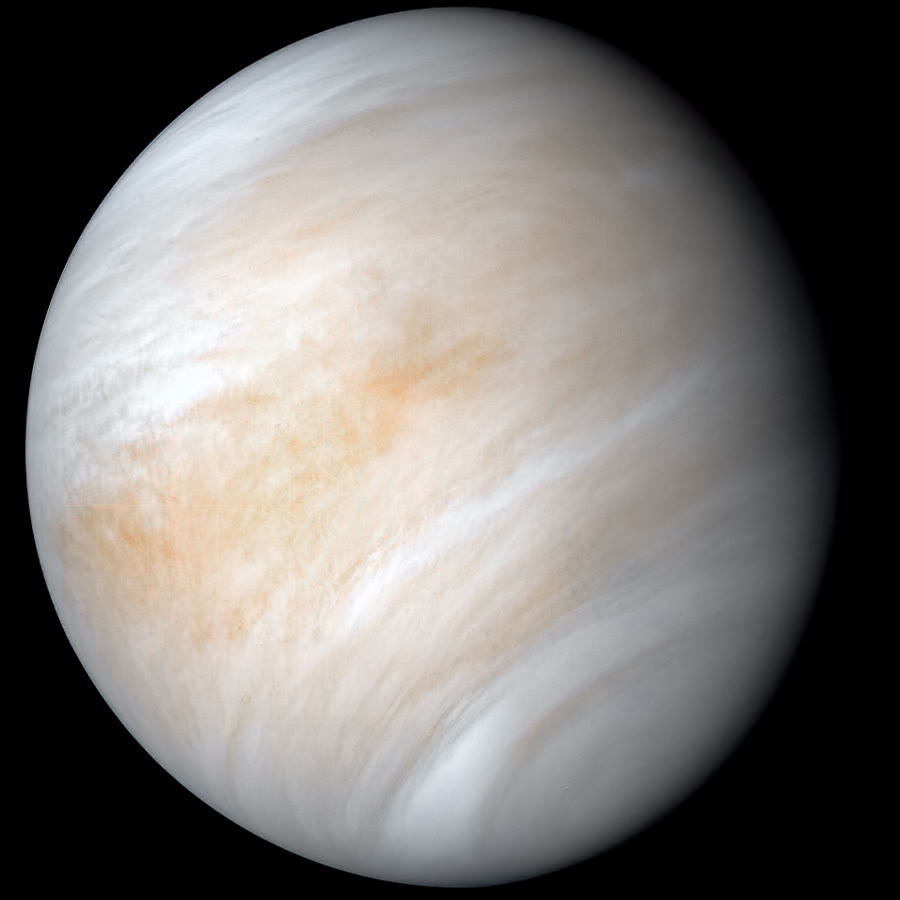
\includegraphics[width=0.38\linewidth]{images/book2/g10-nasa-venus-mariner10.jpg}

{\small الزهرة كما رآها المسبار مارينر~10 عام 1974، بألوان قريبة مما تراه
العين: كوكب يلفّه السحاب كليًّا. الصورة: ناسا/مختبر الدفع النفاث--معهد
كاليفورنيا للتقنية (ملك عام).}
\end{omfigure}

\begin{recall}
الشمس نجم؛ وحولها تدور الكواكب الصخرية الأربعة عطارد والزهرة والأرض والمريخ،
ثم الكواكب العملاقة الأربعة، في مدارات شبه دائرية (كتب الفيزياء والكتاب 1).
وكل جسم يشع طاقة على شكل ضوء، تزداد كلما ارتفعت درجة حرارته، ومعظمها ضوء تحت
أحمر عند درجات حرارة الكواكب (كتب الفيزياء). وغازات الدفيئة --- بخار الماء
وثاني أكسيد الكربون والميثان --- تمتص جزءًا من الأشعة تحت الحمراء التي يطلقها
السطح فتبقيه أدفأ (كتب الكيمياء). ويوجد الماء جليدًا وماءً سائلًا وبخار ماء؛
والضغط قوة لكل وحدة مساحة، ويقاس بالباسكال (كتب الفيزياء).
\end{recall}

\section{درجة الحرارة التي يفرضها النجم}

ترسل الشمس ضوءها بالتساوي في كل الاتجاهات. وعلى مسافة $d$، تتوزع قدرتها $L$
(\emph{ضياؤها}) على كرة مساحتها $4\pi d^2$.

\begin{proposition}[قانون التربيع العكسي لضوء الشمس]\label{prop:g10:habitable-planet:inverse-square}
القدرة التي يتلقاها كل متر مربع مواجه للشمس، وهي \emph{الإشعاعية
الشمسية}، على مسافة $d$ من الشمس هي
\[
  S = \frac{L}{4\pi d^2}.
\]
وعلى مسافة الأرض، \qty{1}{au}، تكون $S_0 = \qty{1361}{W/m^2}$؛ وعلى
مسافة $d$ مقيسة بالوحدات الفلكية، تكون $S = S_0/d^2$.
\end{proposition}

\begin{proof}
لا يضيع أي ضوء في الفضاء الخالي، فالقدرة $L$ كلها تعبر كل كرة مركزها الشمس؛
وعلى كرة نصف قطرها $d$ تتوزع على $4\pi d^2$ مترًا مربعًا. ومضاعفة $d$ تضرب
المساحة في أربعة وتقسم $S$ على
أربعة.
\end{proof}
% ledger: earth:TSI, sun:L, const:au

\begin{omfigure}
\begin{tikzpicture}[font=\small, >={Stealth[length=2mm]}]
  \shade[ball color=yellow!70!orange] (0,0) circle (0.35);
  \node[below=4pt] at (0,-0.35) {الشمس};
  \draw[omThm!70, thick] (0,0) -- (3,0.6) (0,0) -- (3,-0.6);
  \draw[omThm!70, thick, dashed] (3,0.6) -- (6,1.2) (3,-0.6) -- (6,-1.2);
  \draw[fill=omDef!25, draw=omDef!80!black] (3,-0.6) rectangle (3.18,0.6);
  \draw[fill=omDef!12, draw=omDef!80!black] (6,-1.2) rectangle (6.18,1.2);
  \draw[omDef!80!black] (6,0) -- (6.18,0) (6.09,-1.2) -- (6.09,1.2);
  \node[anchor=north] at (3.1,-0.7) {$d$};
  \node[anchor=north] at (6.1,-1.3) {$2d$};
  \node[anchor=south east, align=right, font=\footnotesize] at (2.9,0.75) {\foreignlanguage{arabic}{مربع واحد:}\\كل الضوء};
  \node[anchor=west, align=left, font=\footnotesize] at (6.35,0.6) {\foreignlanguage{arabic}{4 مربعات:}\\ربع لكل منها};
  \draw[->, black!60] (0.5,-1.95) -- (6.1,-1.95);
  \node[anchor=north, font=\footnotesize] at (3.3,-2.0) {البعد عن الشمس};
\end{tikzpicture}

{\small الضوء الذي يعبر مربعًا واحدًا على المسافة $d$ يتوزع على أربعة مربعات
من الحجم نفسه على المسافة $2d$: فالإشعاعية تتناقص بحسب مقلوب مربع
المسافة.}
\end{omfigure}

يمتص الكوكب الجزء الذي لا يعكسه من هذا الضوء، ويشع طاقة نحو الفضاء على شكل ضوء
تحت أحمر. فإذا امتص أكثر مما يشع، سخن؛ وإذا سخن، أشع أكثر؛ فيستقر عند درجة
الحرارة التي يتوازن عندها الأمران.

\begin{definition}[درجة حرارة التوازن]\label{def:g10:habitable-planet:equilibrium-temperature}
\emph{درجة حرارة التوازن}\index{درجة حرارة التوازن} لكوكب هي درجة الحرارة
التي يرسل عندها جسم يشع كباعث مثالي نحو الفضاء القدرة نفسها تمامًا التي
يمتصها الكوكب من نجمه. ويُسمى الكسر الذي يعكسه الكوكب ككل من الضوء الوارد
\emph{ألبيدو بوند} $A$.
\end{definition}

\begin{proposition}[حساب درجة حرارة التوازن]\label{prop:g10:habitable-planet:teq}
لكوكب يوزع الحرارة التي يمتصها على سطحه كله،
\[
  T_{\mathrm{eq}} = \left(\frac{S\,(1-A)}{4\sigma}\right)^{1/4},
  \qquad \sigma = \qty{5.67e-8}{W.m^{-2}.K^{-4}}.
\]
وعلى مسافة الأرض ومن دون أي انعكاس، يعطي هذا
\qty{278.3}{K}؛ وعلى مسافة $d$ بالوحدات الفلكية ومع ألبيدو $A$، تكون
$T_{\mathrm{eq}} = \qty{278.3}{K} \times (1-A)^{1/4}/\sqrt{d}$.
\end{proposition}

\begin{proof}[برهان جزئي]
يعترض الكوكب ضوء الشمس على قرص مساحته $\pi R^2$ ويمتص القدرة
$(1-A)\,S\,\pi R^2$. ويشع من سطحه كله، أي من $4\pi R^2$.
والباعث المثالي عند درجة الحرارة $T$ يشع $\sigma T^4$ لكل متر مربع (وهو قانون
مبرهن في كتب الفيزياء، نقبله هنا). ومساواة
$4\pi R^2 \sigma T^4 = (1-A)\,S\,\pi R^2$ تعطي الصيغة؛ ويختزل نصف القطر.
ومع $S = S_0/d^2$، يكون الجذر الرابع للمقدار $1/d^2$ هو $1/\sqrt d$.
\end{proof}
% ledger: const:sigma, earth:TSI

\begin{example}[الأرض]\label{ex:g10:habitable-planet:earth}
% ledger: earth:TSI, earth:albedo, earth:Tbb, earth:Tsurf
مع $S_0 = \qty{1361}{W/m^2}$ و$A = 0.294$،
$T_{\mathrm{eq}} = 278.3 \times 0.706^{1/4} \approx \qty{255}{K}$، أي
\qty{-18}{\degreeCelsius}. (وتذكر بطاقة بيانات ناسا \qty{254}{K}.) أما متوسط
درجة حرارة سطح الأرض فهو \qty{288}{K}،
\qty{15}{\degreeCelsius}: فأثر الدفيئة في الغلاف الجوي يدفئه بنحو
\qty{33}{K}. ولولاه لتجمدت المحيطات.
\end{example}

\begin{omfigure}
\begin{tikzpicture}
\begin{axis}[ybar, width=0.86\linewidth, height=5.8cm, ymin=0, ymax=950,
  bar width=10pt, enlarge x limits=0.15, symbolic x coords={Mercury,Venus,Earth,Moon,Mars},
  xticklabels={عطارد,الزهرة,الأرض,القمر,المريخ},
  xtick=data, ylabel={\foreignlanguage{arabic}{درجة الحرارة \babelsublr{(K)}}}, ymajorgrids, grid style={gray!22},
  legend style={at={(0.97,0.95)}, anchor=north east, font=\footnotesize, draw=black!30},
  nodes near coords, nodes near coords style={font=\scriptsize, rotate=90, anchor=west, /pgf/number format/fixed, /pgf/number format/precision=0},
  tick label style={font=\small}, label style={font=\small}]
\addplot[fill=omDef!45, draw=omDef!80!black] table[x=name, y=Teq_K] {figdata/out/grade-10-planet_temperatures-planets.dat};
\addlegendentry{درجة حرارة التوازن}
\addplot[fill=omThm!55, draw=omThm!80!black] table[x=name, y=Tmean_K] {figdata/out/grade-10-planet_temperatures-planets.dat};
\addlegendentry{متوسط درجة حرارة السطح المقيس}
\end{axis}
\end{tikzpicture}

{\small \omterm{def:g10:habitable-planet:equilibrium-temperature}{درجات حرارة التوازن} المحسوبة من مسافة كل جسم وألبيدو بوند الخاص به،
بجانب متوسطات درجات حرارة سطوحها المقيسة. البيانات: بطاقات بيانات الكواكب لدى
ناسا.}
\end{omfigure}

\begin{remark}[قراءة المخطط]\label{rem:g10:habitable-planet:reading}
% ledger: nasa:bond-albedos, planet:Mercury.Tmean, planet:Venus.Tmean, planet:Moon.Tmean, planet:Mars.Tmean, planet:Moon.day, nasa:moon-temps
في عطارد والمريخ، اللذين لا غلاف جوي لهما تقريبًا أو لهما غلاف رقيق جدًا،
يقترب المتوسط المقيس من \omterm{def:g10:habitable-planet:equilibrium-temperature}{درجة حرارة التوازن}. أما متوسط القمر فيقع دونها: إذ
يدوم كل من نهاره وليله نحو أسبوعين، ويتأرجح سطحه بين نحو \qty{95}{K} ونحو
\qty{390}{K}، وهو ما لا تلتقطه الصيغة البسيطة الموضوعة لكوكب يوزع حرارته
بالتساوي. والزهرة هي الحالة اللافتة: فمع ألبيدو بوند قدره 0.77 --- إذ تعكس
سحبها معظم ضوء الشمس --- تكون \omterm{def:g10:habitable-planet:equilibrium-temperature}{درجة حرارة توازنها} أدنى من \omterm{def:g10:habitable-planet:equilibrium-temperature}{درجة حرارة توازن}
الأرض، ومع ذلك فسطحها أسخن منها بأكثر من \qty{500}{K}: وذلك أثر الدفيئة في
غلافها الجوي الكثيف من ثاني أكسيد الكربون.
\end{remark}

\section{الاحتفاظ بغلاف جوي}

يتكون الغاز من جزيئات في حركة دائمة، تزداد سرعتها كلما سخن الغاز. والجزيء في
أعلى غلاف جوي الذي يتحرك صعودًا بسرعة تفوق سرعة الإفلات من الكوكب --- وهي
السرعة اللازمة لمغادرة جاذبيته نهائيًا (كتب الفيزياء) --- يضيع في الفضاء. وعلى
مدى مليارات السنين، يفقد الكوكب الصغير ذو الجاذبية الضعيفة هواءه؛ أما الكبير
فيحتفظ به.

\begin{center}
\small
% ledger: planet:Mercury.vesc, planet:Venus.vesc, planet:Earth.vesc, planet:Moon.vesc, planet:Mars.vesc, planet:Mercury.psurf, planet:Venus.psurf, planet:Earth.psurf, planet:Moon.psurf, nasa:mars-atm
\begin{tabular}{lccc}
\hline
الجسم & سرعة الإفلات (\unit{km/s}) & الضغط عند السطح (bar) & الغلاف الجوي \\
\hline
القمر & 2.4 & 0 & لا يوجد \\
عطارد & 4.3 & 0 & لا يوجد \\
المريخ & 5.0 & 0.006 & رقيق، ثاني أكسيد الكربون \\
الزهرة & 10.4 & 92 & كثيف، ثاني أكسيد الكربون \\
الأرض & 11.2 & 1 & نيتروجين وأكسجين \\
\hline
\end{tabular}
\end{center}

\begin{remark}[الحجم ليس كل القصة]\label{rem:g10:habitable-planet:size}
فقد القمر وعطارد، وهما صغيران و(في حالة عطارد) قريبان من الشمس الحارة، كل
غازاتهما تقريبًا. واحتفظ المريخ، الذي تبلغ سرعة الإفلات منه نصف سرعة الإفلات
من الأرض، بغلاف جوي رقيق. أما الزهرة والأرض فلهما الحجم نفسه وسرعة الإفلات
نفسها تقريبًا، ومع ذلك فغلافاهما الجويان مختلفان جدًا: فقد تباعد تاريخاهما ---
مصير مائهما ومصير ثاني أكسيد الكربون فيهما --- كما سيبيّن
\cref{ch:g12:early-earth} في حالة الأرض.
\end{remark}

\section{الماء السائل}

\begin{omfigure}
\begin{tikzpicture}
\begin{axis}[omrecord, width=0.88\linewidth, height=7.2cm, xmin=150, xmax=800,
  ymode=log, ymin=1e-6, ymax=2000, xlabel={\foreignlanguage{arabic}{درجة الحرارة \babelsublr{(K)}}}, ylabel={\foreignlanguage{arabic}{الضغط \babelsublr{(bar)}}},
  xtick={200,300,...,800}, ytick={1e-6,1e-4,1e-2,1,100},
  log basis y=10]
\addplot[omDef!85!black, line width=1.1pt] table[x=T_K, y=p_bar] {figdata/out/grade-10-planet_temperatures-vap.dat};
\addplot[omDef!85!black, line width=1.1pt] table[x=T_K, y=p_bar] {figdata/out/grade-10-planet_temperatures-subl.dat};
\addplot[omDef!85!black, line width=1.1pt] table[x=T_K, y=p_bar] {figdata/out/grade-10-planet_temperatures-melt.dat};
\addplot[only marks, mark=*, mark size=2pt, black] coordinates {(273.16,0.00611657) (647.096,220.64)};
\addplot[only marks, mark=square*, mark size=2.4pt, omThm!85!black] table[x=T_K, y=p_bar] {figdata/out/grade-10-planet_temperatures-points.dat};
\node[font=\small] at (axis cs:205,30) {جليد};
\node[font=\small] at (axis cs:420,30) {سائل};
\node[font=\small] at (axis cs:600,1e-3) {بخار الماء};
\node[font=\footnotesize, anchor=north west] at (axis cs:276,0.0055) {النقطة الثلاثية};
\node[font=\footnotesize, anchor=south east] at (axis cs:640,300) {النقطة الحرجة};
\node[font=\footnotesize, anchor=south, omThm!85!black] at (axis cs:737,110) {الزهرة};
\node[font=\footnotesize, anchor=west, omThm!85!black] at (axis cs:296,1.0) {الأرض};
\node[font=\footnotesize, anchor=north, omThm!85!black] at (axis cs:210,0.0045) {المريخ};
\end{axis}
\end{tikzpicture}

{\small مخطط أطوار الماء، مع متوسط ظروف السطح على الزهرة والأرض والمريخ
(المربعات). ومحور الضغط لوغاريتمي: كل تدريجة تساوي مئة ضعف التي تحتها. حُسبت
المنحنيات من معادلات الرابطة الدولية لخواص الماء والبخار؛ وقيم الكواكب من
ناسا.}
\end{omfigure}

\begin{proposition}[متى يمكن أن يكون الماء سائلًا]\label{prop:g10:habitable-planet:liquid}
% ledger: iapws:triple-critical, iapws:vapour-pressure, iapws:melt-subl
لا يوجد الماء السائل إلا عند ضغوط أعلى من ضغط \emph{النقطة الثلاثية}،
\qty{611.657}{Pa} (\qty{0.006}{bar})، حيث يتعايش الجليد والسائل والبخار
عند \qty{273.16}{K}، وعند درجات حرارة أدنى من \emph{النقطة الحرجة}،
\qty{647.096}{K} (\qty{220.64}{bar})، التي لا يعود ممكنًا بعدها التمييز بين
السائل والبخار. وعند ضغط معين أعلى من النقطة الثلاثية، يكون الماء سائلًا بين
نقطة انصهاره، القريبة من \qty{273}{K}، ونقطة غليانه، التي تنخفض بانخفاض
الضغط.
\end{proposition}

\begin{example}[ثلاثة كواكب على مخطط واحد]\label{ex:g10:habitable-planet:three}
% ledger: nasa:venus-atm, nasa:mars-atm, earth:psurf, earth:Tsurf (boiling point at 636 Pa computed)
يقع سطح الأرض، عند \qty{288}{K} و\qty{1}{bar}، داخل
مجال السائل: فالماء فيه يمكن أن يكون سائلًا أو جليدًا أو بخارًا بحسب الطقس.
وتقع الزهرة، عند \qty{737}{K}، بعيدًا وراء درجة الحرارة الحرجة: فلا ماء سائل
ممكن فيها إطلاقًا. أما المريخ، عند \qty{6.36}{mbar}، فيقع فوق النقطة الثلاثية
بقليل: فالماء فيه يغلي عند نحو \qty{0.5}{\degreeCelsius}، فلا يمكن أن يبقى الماء
السائل إلا في نافذة عرضها نحو نصف درجة، ومتوسط درجة الحرارة،
\qty{210}{K}، يقع في مجال الجليد.
\end{example}

\begin{omfigure}
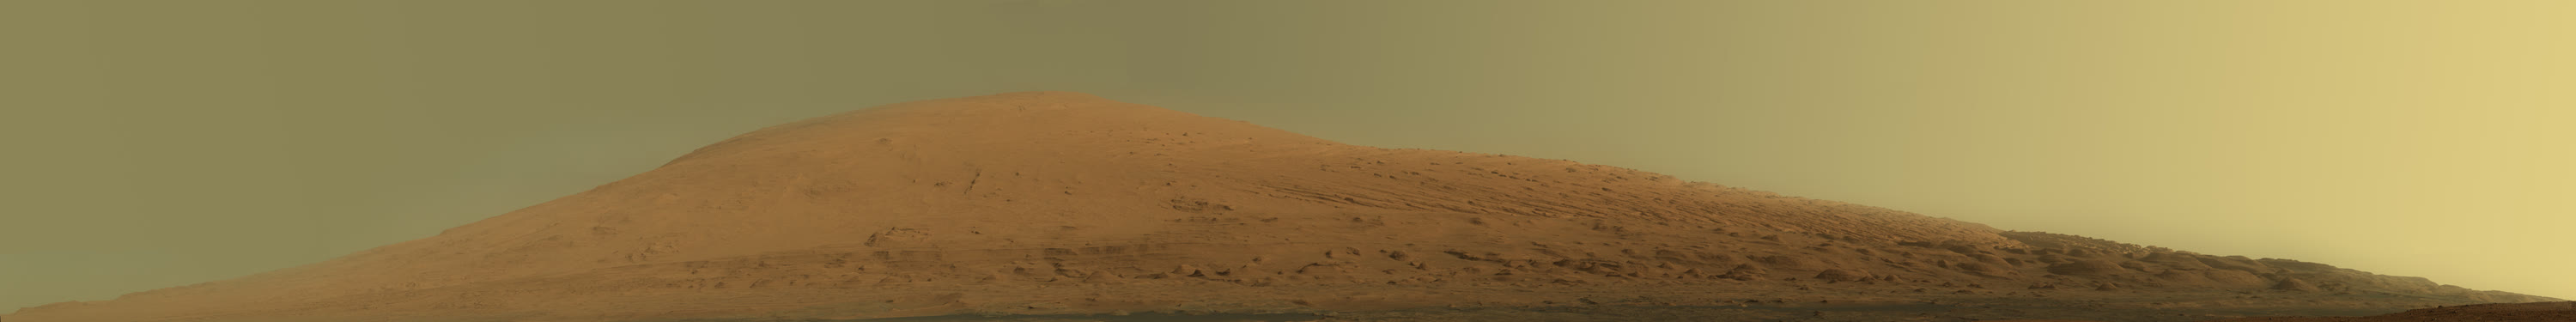
\includegraphics[width=0.96\linewidth]{images/book2/g10-nasa-mars-mount-sharp.jpg}

{\small جبل شارب، داخل فوهة غيل على المريخ، كما صوّرته العربة الجوالة
كيوريوسيتي عام 2012، بالألوان التي سجلتها كاميرتها. وقد ترسّبت طبقاته السفلى
في الماء، قبل مليارات السنين. الصورة: ناسا/مختبر الدفع النفاث--معهد كاليفورنيا
للتقنية/MSSS (ملك عام).}
\end{omfigure}

\section{النطاق الصالح للحياة}

\begin{definition}[النطاق الصالح للحياة]\label{def:g10:habitable-planet:habitable-zone}
\emph{النطاق الصالح للحياة}\index{نطاق صالح للحياة} لنجم هو مجال المسافات عن
النجم التي يستطيع فيها كوكب صخري فيه ما يكفي من الماء وغلاف جوي كغلاف الأرض
أن يحتفظ بماء سائل على سطحه. وحافته الداخلية حيث يفقد الكوكب ماءه بفعل
الحرارة؛ وحافته الخارجية حيث لا يعود حتى أثر دفيئة قوي قادرًا على منعه
من التجمد.
\end{definition}

\begin{proposition}[النطاق الصالح للحياة حول الشمس]\label{prop:g10:habitable-planet:hz-sun}
% ledger: kopparapu:hz-sun, planet:Mercury.dist, planet:Venus.dist, planet:Mars.dist
تضع النماذج المفصّلة للأغلفة الجوية للكواكب النطاقَ الصالح للحياة حول الشمس
بين \qty{0.99}{au} و\qty{1.70}{au}. فالأرض (\qty{1}{au}) تقع داخل حافته
الداخلية بقليل؛ والمريخ (\qty{1.52}{au}) يقع داخله؛ أما الزهرة
(\qty{0.72}{au}) فتقع دون الحافة الداخلية بكثير.
\end{proposition}

\begin{proposition}[النطاقات الصالحة للحياة حول نجوم أخرى]\label{prop:g10:habitable-planet:hz-scaling}
حول نجم ضياؤه $L$، يتلقى الكوكب الإشعاعية نفسها التي يتلقاها على مسافة
$d_\odot$ من الشمس حين يقع على المسافة
\[
  d = d_\odot \sqrt{L/L_\odot}.
\]
وتنتقل حافتا \omterm{def:g10:habitable-planet:habitable-zone}{النطاق الصالح للحياة} بالنسبة نفسها، في تقريب أول (ولون ضوء النجم
له أيضًا أثر طفيف).
\end{proposition}

\begin{proof}
تساوي الإشعاعية يعني $L/(4\pi d^2) = L_\odot/(4\pi d_\odot^2)$، إذن
$d^2 = d_\odot^2\,L/L_\odot$.
\end{proof}

\begin{omfigure}
\begin{tikzpicture}[font=\small]
  % top: the Sun, 0-2 au over 12 cm (6 cm per au)
  \fill[omProp!30] (0.99*6,0) rectangle (1.70*6,0.5);
  \draw[black!70] (0,0.25) -- (12.3,0.25);
  \foreach \x in {0,0.5,...,2} \draw (\x*6,0.15) -- (\x*6,0.35) node[pos=0, below=1pt, font=\footnotesize] {\x};
  \shade[ball color=yellow!70!orange] (0,0.25) circle (0.22);
  \foreach \n/\d in {عطارد/0.387, الزهرة/0.723, الأرض/1.0, المريخ/1.524} {
    \fill[omThm!85!black] (\d*6,0.25) circle (2.2pt);
    \node[anchor=south, font=\footnotesize] at (\d*6,0.55) {\n};
  }
  \node[anchor=west, font=\footnotesize] at (12.4,0.25) {au};
  \node[anchor=north, font=\footnotesize] at (8.07,-0.25) {\foreignlanguage{arabic}{النطاق الصالح للحياة، \babelsublr{0.99--1.70 au}}};
  \node[anchor=east, font=\footnotesize] at (-0.3,0.25) {الشمس};
  % bottom: Proxima Centauri, 0-0.1 au over 12 cm (120 cm per au)
  \begin{scope}[yshift=-2.2cm]
  \fill[omProp!30] (0.0385*120,0) rectangle (0.0661*120,0.5);
  \draw[black!70] (0,0.25) -- (12.3,0.25);
  \foreach \x/\l in {0/0, 0.025/0.025, 0.05/0.05, 0.075/0.075, 0.1/0.1} \draw (\x*120,0.15) -- (\x*120,0.35) node[pos=0, below=1pt, font=\footnotesize] {\l};
  \shade[ball color=red!70!orange] (0,0.25) circle (0.14);
  \fill[omThm!85!black] (0.0485*120,0.25) circle (2.2pt);
  \node[anchor=south, font=\footnotesize] at (0.0485*120,0.55) {بروكسيما ب};
  \node[anchor=west, font=\footnotesize] at (12.4,0.25) {au};
  \node[anchor=north, font=\footnotesize] at (6.28,-0.25) {\foreignlanguage{arabic}{النطاق الصالح للحياة، \babelsublr{0.038--0.066 au}}};
  \node[anchor=east, align=right, font=\footnotesize] at (-0.3,0.25) {بروكسيما\\قنطورس};
  \end{scope}
\end{tikzpicture}

{\small في الأعلى: \omterm{def:g10:habitable-planet:habitable-zone}{النطاق الصالح للحياة} حول الشمس والكواكب الصخرية الأربعة. وفي
الأسفل: \omterm{def:g10:habitable-planet:habitable-zone}{النطاق الصالح للحياة} حول النجم الأحمر الخافت بروكسيما قنطورس، محسوبًا
بتغيير مقياس نطاق الشمس بالجذر التربيعي لضياء النجم، وكوكبه بروكسيما~ب. لاحظ
تغيّر المقياس: فطول الشريط السفلي كله
\qty{0.1}{au}.}
\end{omfigure}

\section{كواكب نجوم أخرى}

\begin{definition}[الكوكب الخارجي]\label{def:g10:habitable-planet:exoplanet}
\emph{الكوكب الخارجي}\index{كوكب خارجي} كوكب يدور حول نجم غير
الشمس.
\end{definition}

الكواكب الخارجية أخفت كثيرًا وأقرب كثيرًا إلى نجومها من أن تُرى مباشرة، باستثناء
بضعة عمالقة. ويُكتشف معظمها بطرق غير مباشرة: فإما أن يمر الكوكب أمام نجمه مرة
في كل دورة فيخفت ضوؤه خفوتًا طفيفًا جدًا، وإما أن تجعل جاذبيته النجم يتمايل
مقتربًا منا ومبتعدًا عنا، فيُزاح لون ضوء النجم ذهابًا وإيابًا. والطريقة الثانية
لا تعطي إلا كتلة \emph{دنيا} للكوكب، لأن ميل المدار غير معروف. وتُدرس هذه
الطرق في مجلد السنة الجامعية الثالثة.

\begin{dated}{2026}
% ledger: nea:count-2026
في 15 أكتوبر 2026 أحصى أرشيف الكواكب الخارجية لدى ناسا \num{6451} كوكبًا
خارجيًّا مؤكَّدًا.
\end{dated}

\begin{example}[بروكسيما ب]\label{ex:g10:habitable-planet:proxima}
% ledger: nea:proxima-b (flux and habitable zone computed in figdata/grade-10/planet_temperatures.py)
أقرب نجم إلى الشمس، بروكسيما قنطورس، على بعد \qty{1.30}{\parsec}، نجم أحمر
صغير لا يتجاوز ضياؤه نحو $0.0015$ من ضياء الشمس. وفي عام 2016 اكتُشف كوكب
يدور حوله كل 11.2 يومًا، على مسافة \qty{0.0485}{au}، كتلته 1.06 مرة كتلة الأرض
على الأقل. وعلى تلك المسافة يتلقى نحو 0.64 من الإشعاعية التي تتلقاها الأرض،
ويقع داخل \omterm{def:g10:habitable-planet:habitable-zone}{النطاق الصالح للحياة} حول نجمه. أما هل له غلاف جوي، أو ماء، فأمر غير
معروف.
\end{example}

\begin{remark}[الصالح للحياة ليس مأهولًا]\label{rem:g10:habitable-planet:inhabited}
\omterm{def:g10:habitable-planet:habitable-zone}{النطاق الصالح للحياة} حكم على المسافة والضوء فقط. فالكوكب الواقع داخله قد لا
يكون فيه ماء، ولا غلاف جوي، أو يكون له غلاف غير مناسب --- فالمريخ يقع داخل نطاق
الشمس وليس على سطحه ماء سائل اليوم. والأرض صالحة للحياة لأن شروطًا عدة تتحقق
فيها معًا: المسافة المناسبة، وكتلة كبيرة بما يكفي للاحتفاظ بغلاف جوي، وماء
وفير، وأثر دفيئة ليس بالضعيف جدًا ولا بالقوي جدًا.
\end{remark}

\section{تمارين}

\begin{exercise}[$\star$]\label{exo:g10:habitable-planet:1}
عرّف \omterm{def:g10:habitable-planet:equilibrium-temperature}{درجة حرارة التوازن} لكوكب. ولماذا يكون متوسط درجة حرارة سطح الأرض أعلى من
\omterm{def:g10:habitable-planet:equilibrium-temperature}{درجة حرارة توازنها}؟
\end{exercise}

\begin{exercise}[$\star$]\label{exo:g10:habitable-planet:2}
باستعمال المخطط العمودي لدرجات الحرارة عند التوازن والمقيسة، سمِّ الجسم الذي
يدفئ غلافه الجوي سطحه أكثر من غيره، وقدّر بكم
كلفنًا.
\end{exercise}

\begin{exercise}[$\star$]\label{exo:g10:habitable-planet:3}
يدور المريخ على بعد \qty{1.52}{au} من الشمس. باستعمال قانون التربيع العكسي مع
$S_0 = \qty{1361}{W/m^2}$، احسب الإشعاعية الشمسية عند المريخ.
\end{exercise}

\begin{exercise}[$\star$]\label{exo:g10:habitable-planet:4}
باستعمال مخطط أطوار الماء، أعطِ حالة الماء عند \qty{1}{bar}
و\qty{330}{K}؛ وعند \qty{0.001}{bar} و\qty{250}{K}؛ وعند \qty{100}{bar}
و\qty{700}{K}.
\end{exercise}

\begin{exercise}[$\star$]\label{exo:g10:habitable-planet:5}
ما \omterm{def:g10:habitable-planet:exoplanet}{الكوكب الخارجي}؟ صِف في جملة واحدة لكل منهما الطريقتين الرئيستين اللتين تُكتشف
بهما الكواكب الخارجية.
\end{exercise}

\begin{exercise}[$\star\star$]\label{exo:g10:habitable-planet:6}
احسب \omterm{def:g10:habitable-planet:equilibrium-temperature}{درجة حرارة توازن} الأرض مع $S_0 = \qty{1361}{W/m^2}$
و$A = 0.294$، ثم مع $A = 0$. وحوّل النتيجتين إلى درجات سلسيوس.
\end{exercise}

\begin{exercise}[$\star\star$]\label{exo:g10:habitable-planet:7}
نجم ضياؤه أربعة أضعاف ضياء الشمس. بين أي مسافتين يقع \omterm{def:g10:habitable-planet:habitable-zone}{النطاق الصالح للحياة}
حوله؟ وهل تقع الأرض، لو وُضعت على بعد \qty{1}{au} منه،
داخله؟
\end{exercise}

\begin{exercise}[$\star\star$]\label{exo:g10:habitable-planet:8}
تدور الزهرة على بعد \qty{0.723}{au}. احسب الإشعاعية التي تتلقاها، ثم \omterm{def:g10:habitable-planet:equilibrium-temperature}{درجة حرارة
توازنها} مع ألبيدو بوند الخاص بها، 0.77. قارن بدرجة حرارة سطحها
\qty{737}{K} وفسّر الفرق.
\end{exercise}

\begin{exercise}[$\star\star$]\label{exo:g10:habitable-planet:9}
يبلغ متوسط الضغط على سطح المريخ \qty{6.36}{mbar}، وهو أعلى بقليل من ضغط النقطة
الثلاثية للماء، ويغلي الماء هناك عند نحو \qty{0.5}{\degreeCelsius}. فسّر لماذا
لا يمكن للماء السائل أن يدوم على سطح المريخ اليوم، حتى في عصر يوم صيفي تبلغ فيه
حرارة الأرض \qty{10}{\degreeCelsius}.
\end{exercise}

\begin{exercise}[$\star\star$]\label{exo:g10:habitable-planet:10}
سرعة الإفلات \qty{2.4}{km/s} على القمر و\qty{11.2}{km/s} على
الأرض. احسب نسبتهما. وفسّر لماذا احتفظت الأرض بغلاف جوي ولم يحتفظ به
القمر.
\end{exercise}

\begin{exercise}[$\star\star$]\label{exo:g10:habitable-planet:11}
افترض أن الأرض غطاها الجليد فارتفع ألبيدو بوند الخاص بها إلى 0.50.
احسب \omterm{def:g10:habitable-planet:equilibrium-temperature}{درجة حرارة توازنها} الجديدة. وفسّر لماذا تميل مثل هذه الحالة، متى بُلغت،
إلى الدوام.
\end{exercise}

\begin{exercise}[$\star\star\star$]\label{exo:g10:habitable-planet:12}
بيّن أن $T_{\mathrm{eq}} = \qty{278.3}{K} \times (1-A)^{1/4}/\sqrt{d}$، حيث
$d$ بالوحدات الفلكية، تنتج من صيغة الفصل. وبأي عامل تتغير \omterm{def:g10:habitable-planet:equilibrium-temperature}{درجة حرارة التوازن}
حين تُضرب المسافة في أربعة؟
\end{exercise}

\begin{exercise}[$\star\star\star$]\label{exo:g10:habitable-planet:13}
على أي بعد من الشمس تكون لكوكب ألبيدوه 0.294 \omterm{def:g10:habitable-planet:equilibrium-temperature}{درجة حرارة توازن} قدرها
\qty{273}{K}؟ قارن بالحافة الداخلية \omterm{def:g10:habitable-planet:habitable-zone}{للنطاق الصالح للحياة}، وفسّر لماذا
تختلفان.
\end{exercise}

\begin{exercise}[$\star\star\star$]\label{exo:g10:habitable-planet:14}
على كوكب ضغط سطحه \qty{1000}{Pa}، يغلي الماء عند نحو
\qty{7}{\degreeCelsius}. بين أي درجتي حرارة يمكن أن يكون الماء سائلًا هناك؟
وماذا يحدث لبحيرة على ذلك الكوكب في يوم تبلغ حرارته
\qty{15}{\degreeCelsius}؟
\end{exercise}

\begin{exercise}[$\star\star\star$]\label{exo:g10:habitable-planet:15}
يدور كوكب على بعد \qty{1.2}{au} من نجم ضياؤه نصف ضياء الشمس.
احسب حافتي \omterm{def:g10:habitable-planet:habitable-zone}{النطاق الصالح للحياة} حول النجم وقل هل يقع الكوكب داخله. وإلى أي
حد يمكن الوثوق بالجواب؟
\end{exercise}

\section{مسألة: هل يستطيع بروكسيما ب أن يحتفظ بمحيط؟}

\begin{problem}[{مسألة نهاية الأسبوع --- من ضوء نجم أحمر خافت إلى درجة حرارة
أقرب كواكبه}]
\label{pb:g10:habitable-planet:1}
% ledger: nea:proxima-b, kopparapu:hz-sun, earth:TSI, earth:albedo, planet:Earth.vesc, nasa:bond-albedos (all results computed in figdata/grade-10/planet_temperatures.py or from the rounded data below)
يقرأ طالب بطاقة بيانات الكوكب بروكسيما~ب. لنجمه ضياء
$L = 0.00151\,L_\odot$؛ ويدور الكوكب على المسافة $d = \qty{0.0485}{au}$
في 11.18 يومًا، وكتلته 1.055 مرة كتلة الأرض على الأقل. استعمل
$S_0 = \qty{1361}{W/m^2}$، و$\sigma = \qty{5.67e-8}{W.m^{-2}.K^{-4}}$، \omterm{def:g10:habitable-planet:habitable-zone}{والنطاق
الصالح للحياة} حول الشمس \qtyrange{0.99}{1.70}{au}، وسرعة الإفلات من الأرض
\qty{11.2}{km/s}.

\medskip
\noindent\textbf{الجزء الأول --- ضوء النجم.}
\begin{enumerate}
  \item احسب الإشعاعية عند الكوكب كسرًا من إشعاعية الأرض،
        $L/d^2$ (حيث $L$ بوحدات ضياء الشمس و$d$ بالوحدات الفلكية).
  \item عبّر عنها بالوحدة \unit{W/m^2}.
  \item قارنها بالإشعاعية عند الزهرة (\qty{2601}{W/m^2}) وعند
        المريخ (\qty{586}{W/m^2}).
  \item كم سنة من سنوات الكوكب تتسع لها سنة أرضية واحدة؟
\end{enumerate}

\medskip
\noindent\textbf{الجزء الثاني --- درجات الحرارة من دون غلاف جوي.}
\begin{enumerate}[resume]
  \item احسب \omterm{def:g10:habitable-planet:equilibrium-temperature}{درجة حرارة التوازن} لكوكب قاتم تمامًا
        ($A = 0$) عند تلك الإشعاعية.
  \item احسبها لكوكب لامع كالزهرة ($A = 0.77$).
  \item أي هاتين الدرجتين أعلى من درجة تجمد الماء؟ وماذا تبيّن النتيجتان عن دور
        السحب والجليد؟
\end{enumerate}

\medskip
\noindent\textbf{الجزء الثالث --- النطاق الصالح للحياة.}
\begin{enumerate}[resume]
  \item احسب $\sqrt{L/L_\odot}$.
  \item احسب الحافة الداخلية \omterm{def:g10:habitable-planet:habitable-zone}{للنطاق الصالح للحياة} حول النجم.
  \item احسب حافته الخارجية.
  \item هل يقع بروكسيما~ب داخل \omterm{def:g10:habitable-planet:habitable-zone}{النطاق الصالح للحياة}؟
  \item على أي بعد من الشمس يتلقى كوكب الإشعاعية نفسها التي يتلقاها
        بروكسيما~ب؟ وأين يقع ذلك من \omterm{def:g10:habitable-planet:habitable-zone}{النطاق الصالح للحياة} حول
        الشمس؟
\end{enumerate}

\medskip
\noindent\textbf{الجزء الرابع --- غلاف جوي وماء؟}
\begin{enumerate}[resume]
  \item لو كان للكوكب متوسط كثافة الأرض، لكان نصف قطره
        $1.055^{1/3}$ مرة نصف قطر الأرض. احسب هذا العامل.
  \item سرعة الإفلات متناسبة مع $\sqrt{M/R}$. قدّر سرعة الإفلات من
        الكوكب. فهل يستطيع الاحتفاظ بغلاف جوي؟
  \item لماذا لا تُعرف الكتلة إلا بوصفها حدًّا أدنى؟
  \item ما أدنى ضغط سطحي يسمح، بحسب مخطط الأطوار، بوجود ماء سائل
        أصلًا؟
  \item احسب \omterm{def:g10:habitable-planet:equilibrium-temperature}{درجة حرارة توازن} بروكسيما~ب مع ألبيدو الأرض،
        0.294.
  \item بكم كلفنًا يجب عندئذ أن يدفئه أثر الدفيئة كي يبلغ سطحه متوسط درجة
        حرارة الأرض،
        \qty{288}{K}؟
\end{enumerate}
\end{problem}
